\ProvidesFile{ch3.tex}[Chapter3]
\chapter{Quantum enhanced localization with a single photon avalanche diode array}
\ix{physics//Physics appendix}

\section{Introduction}

\subsection{A brief introduction to quantum optics}

Experimental techniques have surfaced which take advantage of the quantum nature of light to enhance imaging methods. The advent of very fast and sensitive detectors allows us to measure electromagnetic fields at a timescale where quantum effects can be seen. We often speak of methods such as photon counting or photon statistics, and it is prudent to briefly define the photon and how it can be measured with this technology.

Quantization of the electromagnetic field generally begins by writing a Fourier expansion of solutions to Maxwell's equations called \emph{modes} and identifying the canonical position and momentum variables. This procedure is out of the scope of this thesis. Instead, I start by stating the major result of quantization, in which each mode of the field is quantized as a quantum harmonic oscillator. As such, the Hamiltonian for one particular mode has energy eigenvalues $E_{k} = \hbar\omega_{k}(\hat{n} + \frac{1}{2})$ for mode $k$ with frequency $\omega_{k}$. Since there are potentially infinitely many modes, the wavefunction is $\ket{\psi} = \ket{n_{1},n_{2},...}$ where $n_1$ is the number of photons in the first mode, $n_2$ is the number of photons in the second mode, and so on. The number operator for the $k$-th mode gives $\hat{n}_k\ket{\psi} = n_{k}\ket{\psi}$.

The number operator $\hat{n}_k = \hat{a}_k^\dagger\hat{a}_k$ is defined in terms of operators $\hat{a}_k$ and $\hat{a}_k^\dagger$ which are photon annihilation and creation operators for the $k$-th mode, respectively. These operators satisfy the commutation relations $[\hat{a}_k, \hat{a}_{k'}^\dagger] = \delta_{kk'}$ and $[\hat{a}_k, \hat{a}_{k'}] = [\hat{a}_k^\dagger, \hat{a}_k^\dagger] = 0$. The action of the annihilation and creation operators on the joint number states is:

\begin{equation*}
\hat{a}_k \ket{n_1, n_2, ...} = n_k \ket{n_1, n_2, ...} \;\;
\hat{a}_k^\dagger \ket{n_1, n_2, ...} = (n+1) \ket{n_1, n_2, ...}
\end{equation*}

\subsection{Photon statistics}

\begin{figure*}[t]
\centering
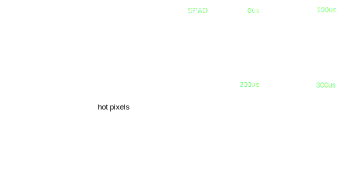
\includegraphics[width=16cm]{/Users/cwseitz/git/cwseitz.github.io/docs/phd/spad/spad/media/Laser-Stats.png}
\caption{\textbf{Poissonian photon statistics of a Gaussian laser spot}. (left) Fano factor plot of pixel-wise variance in photon counts with respect the average photon counts, for 100us exposures of a Gaussian beam pulsed at 10MHz. Equal mean and variance (Poisson statistics) showed as a dashed red line. (right) Example images taken in sequence with the SPAD array.}
\label{fig:fig29}
\end{figure*}    

Using this formalism, we can define any $\ket{\psi}$ that we like in this framework. However, there are certain interesting states which have special properties, such as the coherent state. Coherent states are a special class of states that resemble classical oscillations of the EM field. A coherent state $\ket{\alpha}$ is defined as the eigenstate of the annihilation operator $\hat{a}$:

\begin{equation*}
\hat{a} \ket{\alpha} = \alpha \ket{\alpha}
\end{equation*}

where $\alpha$ is a complex number. The coherent state for a single mode field are given by:

\begin{equation*}
\ket{\alpha} = e^{-\frac{\lvert\alpha\lvert^2}{2}} \sum_{m=0}^\infty \frac{\alpha^m}{m!} \ket{m}
\end{equation*}

It turns out that if we measure a number of photons in this state, we would find that the number of photons has Poisson statistics. To see this, we calculate the probability $p(m)$ of finding $m$ photons in a coherent state $\ket{\alpha}$:

\begin{equation*}
P(m) = \lvert \bra{m} \ket{\alpha} \lvert^2 = \lvert e^{-\frac{\lvert\alpha\lvert^2}{2}} \frac{\alpha^m}{m!} \lvert^2 = e^{-\lvert\alpha\lvert^2} \frac{\lvert\alpha\lvert^{2m}}{m!}
\end{equation*}

This is simply the Poisson distribution with mean $\langle \hat{n} \rangle = \lvert\alpha\lvert^2$. The variance of the photon number distribution in a coherent state is also $\lvert\alpha\lvert^2$, characteristic of Poisson statistics, where the mean and variance are equal. Poissonian fluctuations of a Gaussian beam can be spatially resolved using a single photon avalanche diode (SPAD) array (Figure \ref{fig:fig29}).

In contrast, single photon states e.g, $\ket{1}$ do not necessarily follow Poisson statistics. This state could be prepared by an isolated single photon source such as a fluorescent dye molecule, quantum dot, or nitrogen vacancy, which can produce only a single photon at at time. This phenomenon is referred to as \emph{fluorescence antibunching} where photons tend to be detected as isolated events rather than in bursts or bunches. Single photon sources have a fluorescence lifetime, typically on the order of nanoseconds, which results in a sequence of photon arrivals with a more regular structure than would be expected under Poisson statistics. Note that for such a single photon source the single-mode field can be in state $\ket{1}$ but not state $\ket{2}$ at any given time. If more single photon sources are present or multi-level relaxations occur, states beyond $\ket{1}$ are possible. This has led to the introduction of binomial states of the quantized field \parencite{Stoler1985}. This fact is leveraged in the following sections, to count the number of single photon sources in a region of interest using a widefield photon counting camera.

\section{Second order coherence}

The second-order coherence function, $ g^{(2)}(\tau) $, is a fundamental tool in quantum optics, providing insight into photon statistics without the detailed structure of the field. It can be expressed in terms of the photon count rate $ n(t) $ as:

\begin{equation}
g^{(2)}(\tau) = \frac{\langle n(t) n(t+\tau) \rangle}{\langle n(t) \rangle^2}
\end{equation}

This formulation highlights how the intensity correlations between photons detected at times $ t $ and $ t+\tau $ are normalized by the square of the mean photon count rate, providing a dimensionless measure of the correlation.

The value of $ g^{(2)}(\tau) $ and its dependence on $ \tau $ reveal essential characteristics of the light source. For sub-Poissonian statistics, $ g^{(2)}(0) < g^{(2)}(\tau) $, indicating photon antibunching, where the likelihood of detecting two photons in quick succession is reduced. This behavior is closely related to the fluorescence lifetime of the emitters; after emitting a photon, a fluorophore requires a characteristic time to re-enter the excited state, leading to a dip in $ g^{(2)}(\tau) $ at short $ \tau $. Specifically, at delays much shorter than the fluorescence lifetime, coincidences are unlikely, causing $ g^{(2)}(\tau) $ to approach zero in sub-Poissonian statistics. Poissonian statistics, typical of coherent light, show no correlation between photon arrival times, resulting in $ g^{(2)}(\tau) = 1 $ for all $ \tau $. Super-Poissonian statistics, seen in thermal light, exhibit photon bunching, where $ g^{(2)}(\tau) $ starts high at $ \tau = 0 $ and decays to 1 as $ \tau $ increases, indicating a higher probability of photons arriving close together in time.

The different regimes of $ g^{(2)}(\tau) $ reflect the underlying quantum properties of the light. Thermal light, which follows Bose-Einstein statistics, demonstrates photon bunching due to the collective behavior of photons, leading to a high $ g^{(2)}(0) $. Coherent light, such as that from a laser, exhibits Poisson statistics, where photon arrival times are completely random. Non-classical light sources, particularly single-photon emitters, show sub-Poissonian statistics with photon antibunching, directly related to the fluorescence lifetime. Techniques like Time-Correlated Single Photon Counting (TCSPC) and Hanbury Brown and Twiss (HBT) interferometry are employed to measure $ g^{(2)}(\tau) $, offering profound insights into the quantum nature of light. By analyzing $ g^{(2)}(\tau) $, one can infer properties such as the number of fluorescent emitters in a sample and the temporal dynamics of photon emission processes. In the following section, we will build upon this notion in the context of widefield photon counting. 


\section{Quantum enhanced localization microscopy}

Far-field optical microscopy is fundamentally limited by diffraction, with the maximum attainable resolution being limited to approximately half the wavelength of light. Several schemes to beat the diffraction limit have been developed in recent years. Many of these schemes utilize the concept of precise localization of isolated fluorescent emitters which blink over a time series of frames \parencite{Rust2006,Betzig2006}. An inherent problem with such methods is the requirement that fluorescent emitters be isolated, slowing down the acquisition of super-resolved images. To address this, we leverage the fact that many fluorophores are intrinsically single photon sources and exhibit fluorescence antibunching. This property can constrain the number of active fluorescent emitters in a region of interest (ROI) and can potentially enable localization in non-sparse scenes \parencite{Ta2010,Israel2017}. 

\begin{figure*}[t]
\centering
\includegraphics[width=14cm]{/Users/cwseitz/git/cwseitz.github.io/docs/phd/spad/spad/media/Dark.png}
\caption{\textbf{Dark counts of the SPAD array}. (left) Average pixel-wise dark counts for a 100x100 pixel region exposed for 100ms (right) Variance of dark counts for 100ms exposure.}
\label{fig:fig30}
\end{figure*}    


\begin{figure*}[t]
\centering
\includegraphics[width=14cm]{/Users/cwseitz/git/cwseitz.github.io/docs/phd/spad/spad/media/SPADvCMOS.png}
\caption{\textbf{Comparison of quantum dot images between CMOS and SPAD cameras}. (left) SPAD image of Qdot655 coated on a glass coverslip using a 100X/1.4NA oil-immersion objective (Nikon) and a 10ms exposure time. (right) CMOS image of Qdot655 using a 60X/1.4NA oil-immersion objective (Olympus) and a 10ms exposure time. Both use continuous-wave 640nm excitation}
\label{fig:fig4}
\end{figure*}    

Molecular counting with fluorescence antibunching has a fairly simple motivation: coincidence of photons at multiple detector elements during high speed imaging provides evidence for the number of single photon sources present in the imaged region. Combining the ideas of conventional super-resolution approaches with photon statistics may prove to be a powerful set of methods for bioimaging. SPAD cameras achieve orders of magnitude higher temporal resolutions than standard CMOS cameras, single photon sensitivity, and dark count rates less than 25cps (Figure \ref{fig:fig30}). Furthermore, the reduced readout noise and large fill-factor of recently commercialized SPAD arrays suggests their use for single molecule localization with reduced localization uncertainty.

\begin{figure*}[t]
\centering
\includegraphics[width=14cm]{/Users/cwseitz/git/cwseitz.github.io/docs/phd/spad/spad/media/SPAD512.png}
\caption{\textbf{Experimental setup for widefield photon counting}. A 532nm pulsed laser is directed through a spatial filter, galvo mirror, and passed through filtering and focusing optics to a 100X oil-immersion objective. Emission light of a 50um grid is projected onto the SPAD512 camera (inset)}
\label{fig:fig5}
\end{figure*}    


In this study, we present a method for widefield single photon counting in order to rigorously count fluorophores in the sample and subsequently constrain single molecule localization. We investigate the theoretical properties of the zero-lag second-order coherence function $g^{(2)}(0)$ for widefield photon counting and its spatial properties (Figure \ref{fig:fig5}). Using Bayesian analysis, we derive a posterior distribution on the number of active fluorescent emitters in a region of interest. We then combined this with single molecule localization algorithms and demonstrate resolution of multiple emitters using a multi-emitter fitting algorithm and report localization errors with respect to the Cramer-Rao bound.

\subsection{Basic Scheme}

\begin{figure*}[t]
\centering
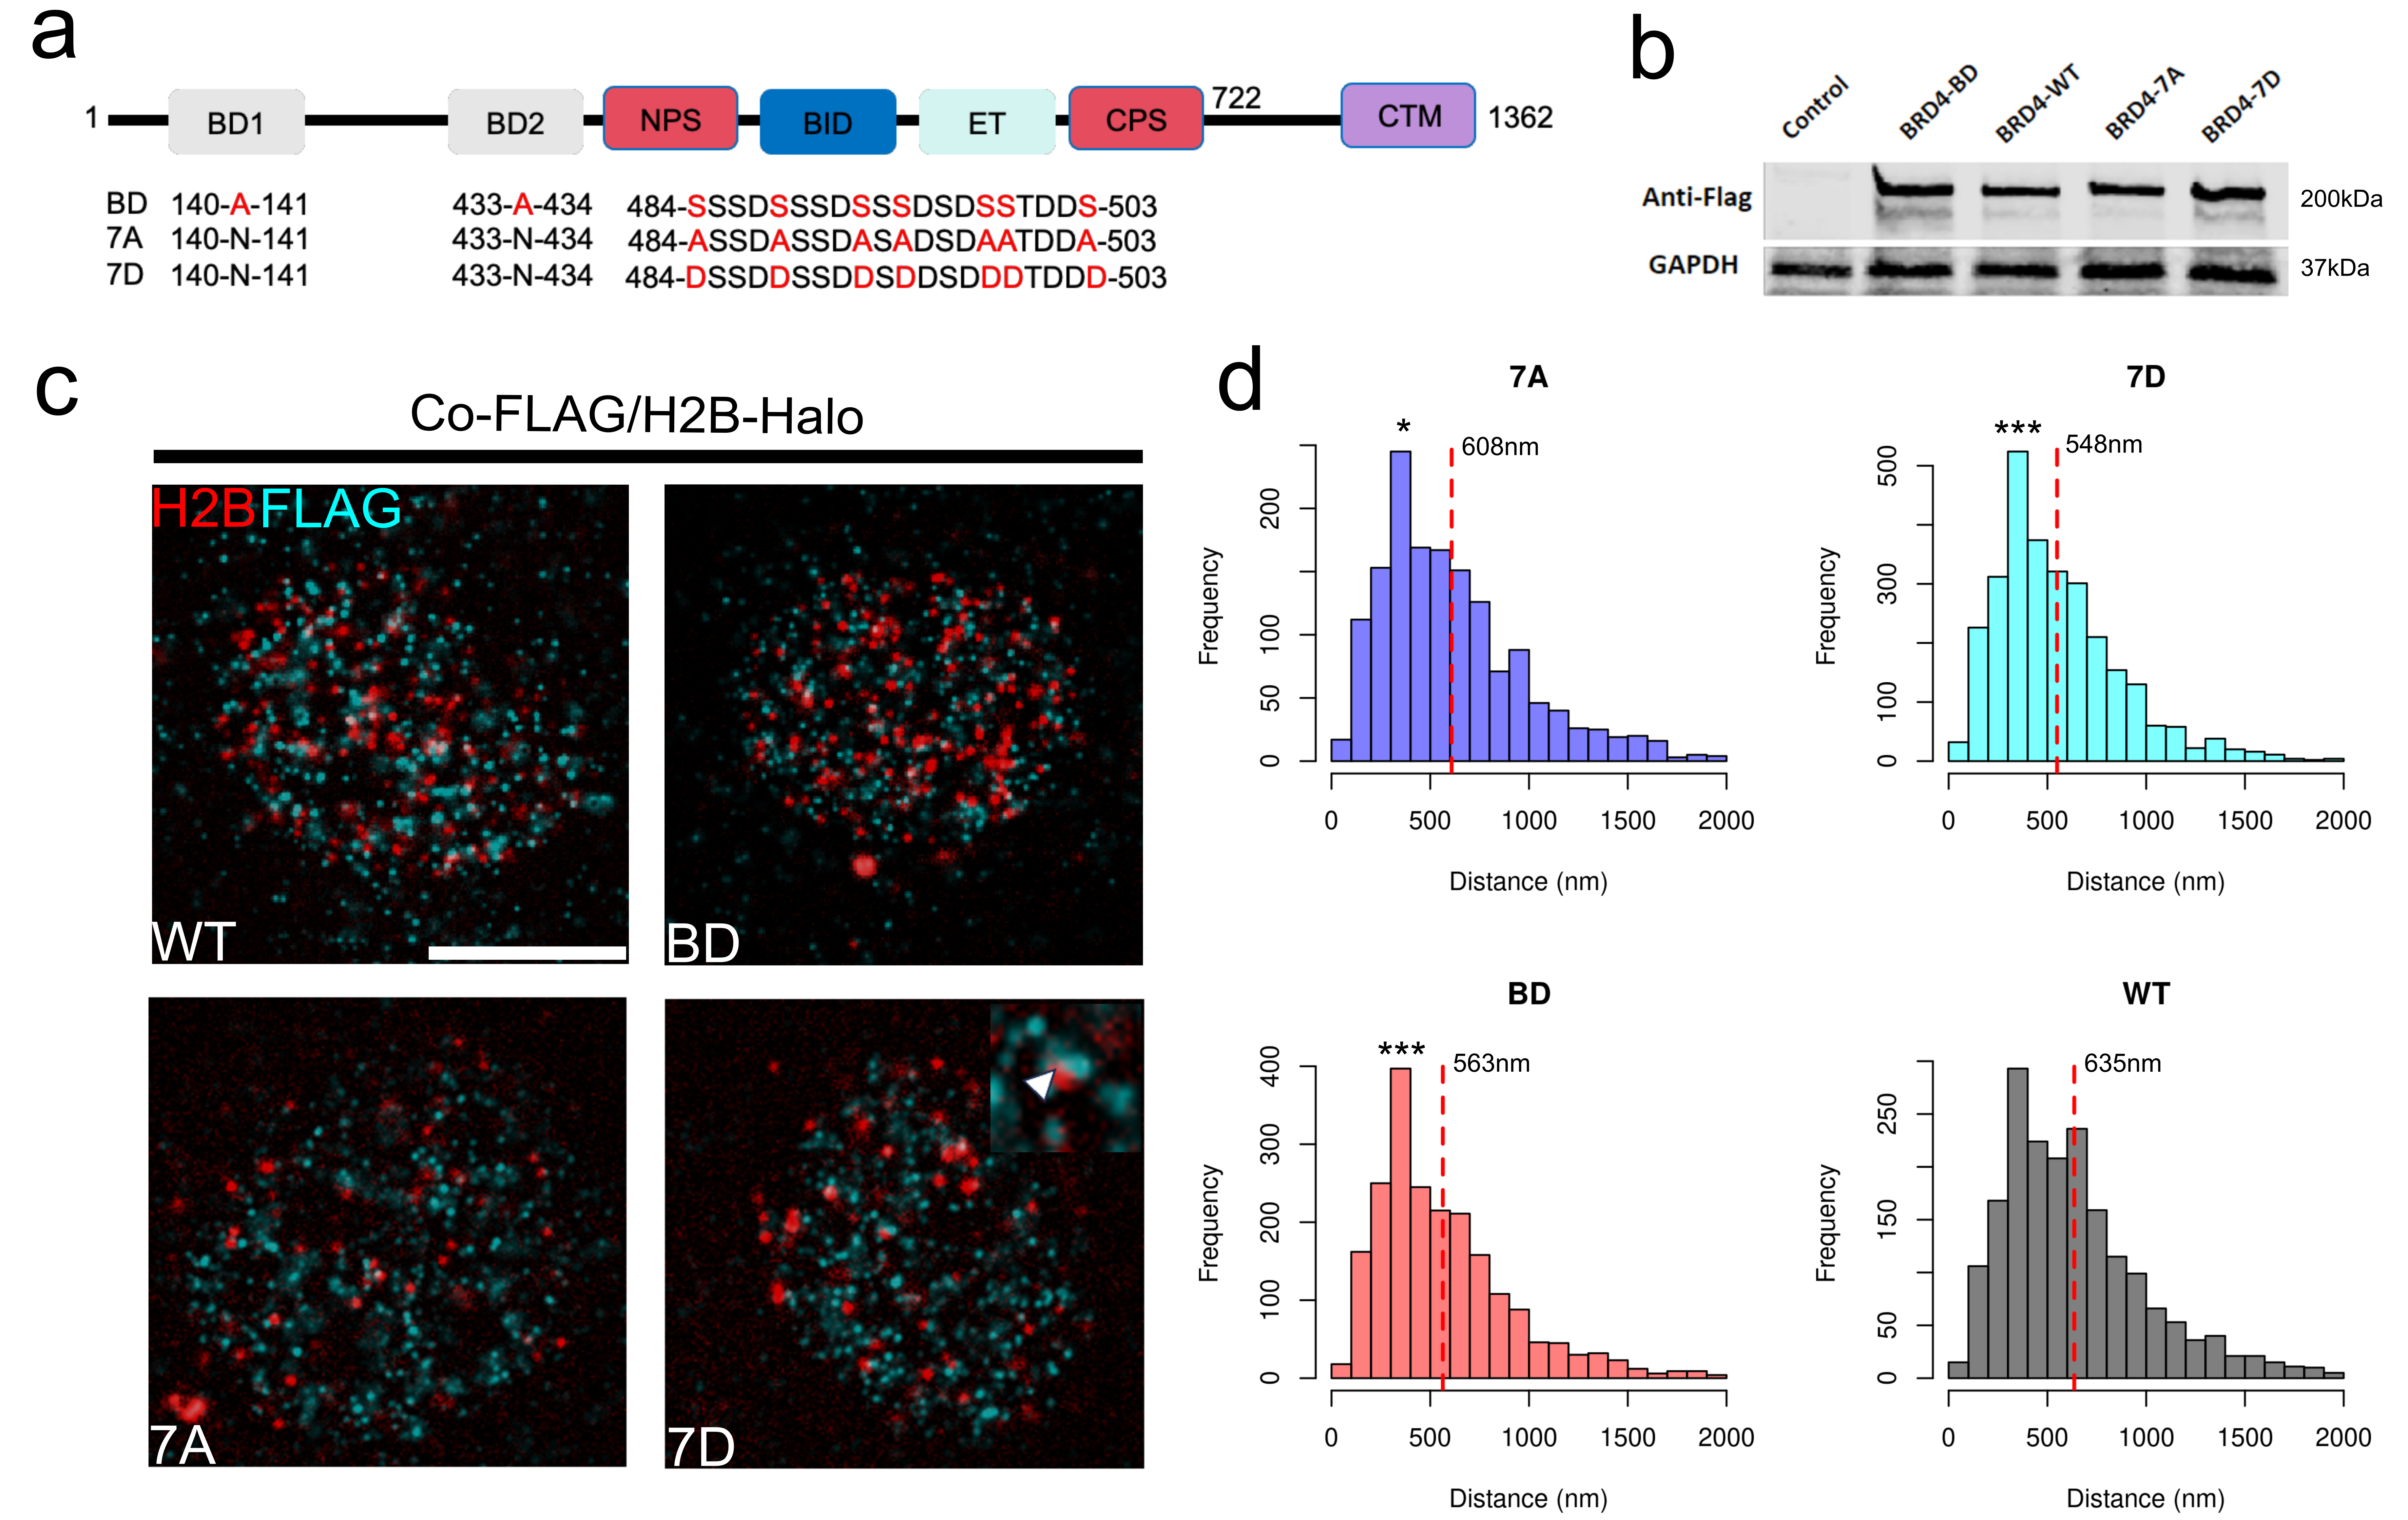
\includegraphics[width=16cm]{/Users/cwseitz/git/cwseitz.github.io/docs/phd/spad/spad/media/Figure-0.png}
\caption{\textbf{Single photon counting with a SPAD array} (a) Conventional widefield microscopy with integrated SPAD array (b) Single photon imaging scheme using 1us exposures containing a picosecond laser pulse (c) Sum of photon counts over a 5x5 region of interest (ROI), taken with $N_{\mathrm{frames}}=5\times 10^{5}$}
\label{fig:fig5}
\end{figure*}    

We consider a simplified description of widefield photon counting for a a single photon source in the object plane labeled by a continuous-valued coordinate $\theta=(\theta_u,\theta_v)$. The spatial profile $O$ of the field in image space is again presumed to have a Gaussian shape \parencite{Zhang2007,Richards1959,Gibson1989}. 

\begin{equation}
O(u,v) = \frac{1}{2\pi\sigma^{2}}e^{-\frac{(u-\theta_u)^2+(v-\theta_v)^2}{2\sigma^2}}
\end{equation}

A similar theoretical exposition to follows to Section 1.2; however, slight modifications are made to the theory to relate it to the quantum theory. Since our SPAD detectors at the image plane must also be discrete, the total field at a detector element $k$ centered in image space at $s_k=(u_k,v_k)$ is then given by integrating over pixels of width $\delta=1$. Using the definitions of $\Gamma_x,\Gamma_y$ from Section 1.2, we define

\begin{equation}
\zeta_{k}\vcentcolon = \langle n_{k} \rangle = \Gamma_{x}(u_k,\theta_u)\Gamma_{y}(v_k,\theta_v)\zeta
\end{equation}

where $\langle n_{k} \rangle$ is the expected number of photons detected at pixel $k$. We now consider the case of pulsed excitation where the interval between pulses much longer than the fluorescence lifetime. Upon excitation of an isolated fluorescent emitter, a photon is detected at a particular detector element $k$ with probability $\zeta_{k}$. Similarly, the probability of detection in a region of interest collecting all photons emitted is $\zeta$. Here, we are primarily concerned with the latter quantity, and its application in counting fluorescent emitters.

\begin{figure}[t]
\centering

\includegraphics[width=12cm]{/Users/cwseitz/git/cwseitz.github.io/docs/phd/spad/spad/media/Figure-4.png}
\caption{\textbf{Posteriors on the number of fluorescent emitters $N$ and localization for $N^{*}=1$} (left) and $N^{*}=2$ (right) quantum dots. Scalebars 360nm}
\label{fig:fig7}
\end{figure}   

By temporarily ignoring the spatial profile described by (1), we derive a likelihood on the number of fluorophores in a small ROI with a lateral dimension $d = 5$ pixels. For $N$ fluorophores emitting photons which can be detected within a ROI of the SPAD array, the number of signal photons measured $n_{\mathrm{signal}}$ following a single excitation pulse will have Binomial statistics $n_{\mathrm{signal}} \sim \mathrm{Binom}(N,\zeta)$. Photon pile-up at a single detector element can be safely neglected in this model due to its relatively low likelihood. We then model the background signal within the region of interest as a coherent state, which we have shown followd Poissonian statistics $n_{\mathrm{background}} \sim \mathrm{Poisson}(\lambda)$ for an expected number $\lambda$ of background counts in the ROI per frame. The total number of counts $n=n_{\mathrm{signal}}+n_{\mathrm{background}}$ detected in the region of interest following a single pulse is then distributed by the likelihood

\begin{equation}
p(m \mid N,\zeta,\lambda) = \sum_{i=0}^{\infty} \binom{N}{i} \zeta^i (1-\zeta)^{N-i} \frac{\lambda^{m-i}}{(m-i)!} e^{-\lambda}
\end{equation}

The expression in (2) represents a convolution of Poisson and Binomial probability mass functions. This result is the primary means of inference of the number of active emitters $N$ in a ROI.

In order to begin to perform localization in non-sparse ROIs, we write a posterior distribution on the Binomial parameters used in the likelihood (2) using Bayes rule. When $\lambda$ is known, we have

\begin{equation}
p(N,\zeta\lvert x) \propto p(x\lvert N,\zeta)p(\zeta)
\end{equation}

We use a Gaussian prior on $\zeta$ i.e., $p(\zeta) = \mathcal{N}(\mu_{\zeta},\sigma_{\zeta})$ with $\mu_{\zeta}=0.01$ and $\sigma_{\zeta}=0.005$. Prior uncertainty in the value of $\zeta$ stems from fluorophores with potentially heterogeneous photophysical properties as well as varying laser power throughout the excited region. This posterior can be integrated over $\zeta$ to produce a posterior distribution on the fluorophore number $N$ i.e., $p(N=N'\lvert n) \propto \int_{0}^{1} \prod_{j=1}^{N\mathrm{frames}} p(n_{j}\lvert N',\zeta)p(\zeta) d\zeta$ which can be estimated using Monte Carlo methods. Monte Carlo integration is employed to integrate out $\zeta$. This involves sampling many $\zeta$ values from the Gaussian prior. For each sampled $\zeta$, the Poisson-Binomial likelihood $p(n\lvert\zeta_i)$ is computed. These likelihood values are then weighted by the prior probabilities $p(\zeta)$. The final result is obtained by averaging these weighted likelihoods over all sampled $\zeta$, which approximates the integral:

\begin{equation*}
\int p(x\lvert\zeta) p(\zeta) \, d\zeta \approx \frac{1}{M} \sum_{i=1}^N p(x\lvert\zeta_i) p(\zeta_i)
\end{equation*}

where $M$ is the number of samples from the prior. This method provides a powerful way to handle the integration of complex or high-dimensional functions, especially when analytical solutions are intractable.

The final posterior is then estimated by minibatching the data into batches of $10^3$ frames and averaging the posterior $p(N\lvert n)$ over minibatches. The fluorophore number $N$ within each ROI is then estimated by the maximum aposteriori (MAP) estimate $N^{*}$ given by this distribution.

For localization, we notice that (2) is well approximated by a Poisson distribution for a large frame number, making the localization procedure similar to conventional maximum likelihood methods discussed in Chapter 1. Therefore, we have the following log-likelihood


\begin{align}
\ell(n\lvert \theta) &= -\log \prod_{k} \frac{e^{-\left(\mu_{k}\right)}\left(\mu_{k}\right)^{n_k}}{n_k!}\\
&= \sum_{k}  \log n_k! + \mu_{k} - n_k\log\left(\mu_{k}\right)
\end{align}

\begin{figure*}[t]
\centering

\includegraphics[width=12cm]{/Users/cwseitz/git/cwseitz.github.io/docs/phd/spad/spad/media/Figure-5.png}
\caption{\textbf{Single and multi-emitter localization error on sums of photon counts}. (left) Localization uncertainty for simulated data for different values of $N$, plotted with respect to the Cramer-Rao lower bound, shown in dashed gray. (right) Multi-emitter localization by MCMC sampling for $N=3$, colors indicate a cluster of samples i.e., a single localization. All data was generated with a background rate $\langle n_{\mathrm{background}} \rangle = \lambda N_{\mathrm{frames}}/d^{2}$ per pixel. Scalebar 360nm}
\label{fig:fig6}
\end{figure*}   

where, in the multi-emitter regime the expected photon count at a pixel is $\mu_{k} = \sum_{m=1}^{N^{*}} \mu_{k,m}$ and $\mu_{k,m}=\zeta N_{\mathrm{frames}}\Gamma_{x}(u_k,\theta_{u,m})\Gamma_{y}(v_k,\theta_{v,m}) + \lambda N_{\mathrm{frames}}/d^{2}$. In the multi-emitter regime, optimization of the likelihood can be more challenging, and sampling is a more suitable choice (see Results). 


\subsection{Results}

Quantum dots coated on a glass coverslip were excited using a picosecond $532\mathrm{nm}$ pulsed laser triggered at $500\mathrm{kHz}$. Emission light was collected using an oil-immersion 100$\times$ objective with numerical aperture (NA) 1.4 (Nikon). The emission signal was then filtered to exclude the laser line (Semrock) and projected onto the SPAD512 sensor (Pi Imaging Technologies) using a tube lens. A simplified diagram of the complete system is depicted in (Figure \ref{fig:fig5} a). Each acquisition consists of $N=5\times 10^{5}$ frames, synchronized with each laser pulse, using a $1\mathrm{us}$ exposure per frame (Figure \ref{fig:fig5} b,d). Example posteriors and multi-emitter fitting on experimental quantum dot data are found in (Figure \ref{fig:fig7}). To confirm the presence of single photon sources in the sample, we investigated properties of the zero-lag second order coherence function $g^{(2)}(0)$. The following empirical estimate of $g^{(2)}(0)$ is used \parencite{Israel2017}

\begin{equation}
g^{(2)}(0) = \frac{G^{(2)}(0)-B}{\langle G^{(2)}(m\neq 0)\rangle -B}
\end{equation}

\begin{figure}[t]
\centering

\includegraphics[width=12cm]{/Users/cwseitz/git/cwseitz.github.io/docs/phd/spad/spad/media/g20g2m.png}
\caption{\textbf{Theoretical scaling of $g^{(2)}(0)$ under zero background conditions}. (left) Scaling of $g^{(2)}(0)$ for small $N$. (right) Scaling of $g^{(2)}(0)$ for large $N$}
\label{fig:fig8}
\end{figure}   

where $B = N_{\mathrm{frames}}\lambda\zeta$ is the expected number of background-signal coincidences in the region of interest. The quantity $G^{(2)}(m)$ represents the number of signal-signal coincidences in the region of interest at a lag time $m$. The quantity $\langle G^{(2)}(m\neq 0)\rangle$ is the average number of coincidences in pairs of frames at nonzero lag $m \in [1,100]$, in units of frames. As expected, simulation from the likelihood (2) shows saturation of $g^{(2)}(0)$  with increasing values of $N$ (Figure \ref{fig:fig5}c). Averaging $G^{(2)}(0)$ over many realizations (sequences of $N_{\mathrm{frames}}$), gives the expected value $\langle G^{(2)}(0)\rangle $

\begin{equation}
\langle G^{(2)}(0)\rangle = N_{\mathrm{frames}}(1 - (1-\zeta)^n - n\zeta (1-\zeta)^{n-1})
\end{equation}

Since $G^{(2)}(m)$ is already averaged over $m$, $\langle G^{(2)}(m) $ is effectively a constant over realizations, and must be

\begin{equation}
\langle G^{(2)}(m)\rangle =  N_{\mathrm{frames}} \left(1 - \left((1-\zeta)^n\right)\right)^2
\end{equation}

Ignoring the effect of background signal $\langle g^{(2)}(0)\rangle =\langle G^{(2)}(0)\rangle/\langle G^{(2)}(m)\rangle$, which rapidly approaches $1/2$ as a function of $N$, and then saturates and very slowly approaches its maximum value of 1 (Figure \ref{fig:fig8}). This is consistent with the idea that for very large number of active fluorescent emitters, the statistics should become Poisson. Moreover, bright clusters of quantum dots exhibit elevated $g^{(2)}(0)$ values as can be seen in maps of the $g^{(2)}(0)$ computing using a sliding window over the array (Figure \ref{fig:fig5} e). Lastly, $G^{(2)}(0),G^{(2)}(m),B$ all will have Binomial statistics, which can approximated as Poisson for large N, small p. Error estimation $\delta G^2(0) = \sqrt{G^2(0)}, \delta E(G^2(m)) = \sqrt{\frac{E(G^2(m))}{M}}, \delta B = \sqrt{B}$.

\begin{equation}
\sigma = \text{RMSE}[g^{(2)}(0)] = \sqrt{
    \left[
    \frac{\partial g^{(2)}(0)}{\partial B} \delta B
    \right]^2 +
    \left[
    \frac{\partial g^{(2)}(0)}{\partial \langle G^{(2)} \rangle} \delta \langle G^{(2)} \rangle
    \right]^2 +
    \left[
    \frac{\partial g^{(2)}(0)}{\partial G^{(2)}(0)} \delta G^{(2)}(0)
    \right]^2
}
\end{equation}

We then integrate a Gaussian with this $\sigma$ below the threshold $g^{(2)}(0)=0.5$ as shown in (Figure \ref{fig:fig5} e).

For localization by optimization of (4), we use Goodman and Weare's Markov Chain Monte Carlo (MCMC) algorithm \parencite{Goodman2010} to sample from the posterior on fluorophore locations. In all simulations we assume a uniform prior on coordinates over the ROI and $\zeta$ is known and identical over fluorophores. Fluorophore locations can then be estimated from the posterior samples by K-means clustering of the $(\theta_u,\theta_v)$ coordinates of the first particle and identification of cluster centers. To validate our estimator, we compare its RMSE to the single emitter Cramer-Rao lower bound  (Figure \ref{fig:fig6}).

We find that for thousands of expected signal photon counts, localization uncertainty lies in an acceptable range for localization microscopy (Figure \ref{fig:fig6}). The $\zeta$ value is treated as unknown but homogeneous across fluorophores in the ROI. 

\begin{figure*}[t]
\centering
\includegraphics[width=14cm]{/Users/cwseitz/git/cwseitz.github.io/docs/phd/spad/spad/media/PoissonBinomialPost-1.png}
\caption{\textbf{Posterior distributions of the fluorophore number}. Samples from the Poisson-Binomial convolution distribution using $\zeta=0.01$ for various values of $\lambda$ and $N=1,3,5$ were simulated. The variable $\zeta$ was integrated out by Monte Carlo integration, sampling 1000 $\zeta$ values from the posterior distribution (see main text for details)}
\label{fig:fig9}
\end{figure*}    

\begin{figure*}[t]
\centering
\includegraphics[width=14cm]{/Users/cwseitz/git/cwseitz.github.io/docs/phd/spad/spad/media/PoissonBinomialPost-2.png}
\caption{\textbf{Posterior distributions of the fluorophore number}. Samples from the Poisson-Binomial convolution distribution using $\zeta=0.01$ for various values of $\lambda$ and $N=7,9,11$ were simulated. The variable $\zeta$ was integrated out by Monte Carlo integration, sampling 1000 $\zeta$ values from the posterior distribution (see main text for details)}
\label{fig:fig10}
\end{figure*}    

\begin{figure*}[t]
\centering

\includegraphics[width=14cm]{/Users/cwseitz/git/cwseitz.github.io/docs/phd/spad/spad/media/G2.png}
\caption{\textbf{Example $G^{(2)}(m)$ functions}. Example quantum dot images and respective $G^{(2)}(m)$ functions, taken with 1us frames 500kHz laser repetition rate.}
\label{fig:fig32}
\end{figure*}    

\subsection{Discussion}

Fluorescence intermittency can affect the observed photon-number fluctuations and could be expected to affect the value of $g^{(2)}(0)$ or the posterior on the number of active fluorescent emitters. However, the signal photon number per frame will follow Binomial statistics even in the presence of blinking, the only consequence of which is an effective reduction of the detection probability $\zeta$. If the effect of censoring photons by blinking and lowering the quantum yield can be accounted for, the technique used here may be compatible with common super-resolution techniques such as stochastic optical reconstruction microscopy (STORM). 

The acquisition times necessary to obtain sufficient photon counts for computing the necessary statistics can potentially be very short. Most fluorophores have relaxation times in the nanosecond range and thus photons can be collected at a rate of at tens of millions of excitation pulses per second. These rates are currently difficult to obtain, however, due to limitations in detector throughput. The SPAD camera used in this study has a minimum exposure time in the microsecond range. Furthermore, the data volume can quickly become intractable due to the need for several thousands of frames for a millisecond-scale exposure time. This is currently a complication for techniques like STORM and advancements in the automation for data acquisitions are necessary. The speed of MCMC based localization remains a limitation for post-processing, and optimization of the processing time for localization is left for future work. 

In conclusion, we propose a single molecule imaging technique that allows for simultaneous counting of localization of fluorescent molecules by modeling the quantum properties of fluorescence emission. The technique does not require a nonclassical light source and is designed to supplement standard single molecule localization microscopy techniques. The proposed method can be implemented with a standard widefield fluorescence microscope.

\section{Future directions: quantum illumination strategies}

In recent years, novel quantum illumination strategies have leveraged spatial correlations between downconverted photon pairs to demonstrate the first quantum illumination full-field imaging protocol. These spatial quantum correlations are generated by a nonlinear optical process referred to as spontaneous parametric downconversion (SPDC). SPDC is typically realized using a nonlinear crystal such as Beta Barium Borate (BBO) or $\beta$-BaB$_2$O$_4$. BBO crystals are highly anisotropic and exhibit nonlinear optical properties, which means that polarization of the crystal varies nonlinearly with electric field strength. This nonlinear behavior can lead to a number of useful effects such as second harmonic generation, third harmonic generation, or SPDC \parencite{Boyd2020}. In the SPDC process, a pump photon typically in the ultraviolet range is downconverted into a pair of lower-energy photons, with wavelengths in the visible range. These photons are known as signal and idler photons. This process is a purely quantum mechanical one, and the daughter photons born in this process possess useful quantum mechanical properties. Indeed, physical principles such as conservation of energy and momentum require that the daughter photons born in this nonlinear process are spatially entangled in several degrees of freedom \parencite{Boyd2020}. 


A relatively straightforward application of SPDC is prediction of photon arrival times of the signal beam by measurement of the idler beam with a single photon sensitive detector. For example, this has been applied to improve the signal-to-noise ratio for measuring the absorption of objects through sub–shot-noise measurements \parencite{Brida2010} or imaging through detector noise and background signal \parencite{Gregory2020,Wolley2022}. In such applications, twin beams produced through the SPDC process are directed to different regions of a spatially resolved detector such as a CCD camera or single-photon avalanche diode (SPAD) array detector. By performing a pixel-by-pixel AND-operation between two regions of the array detector containing the SPDC beams, we can preferentially select correlated photon-pair events and reject uncorrelated background light and sensor noise events. Heralding photons using the signal and idler beams involves detecting one photon (either the signal or idler) and using this detection to infer the presence of its entangled counterpart. This method enhances the precision of photon detection and significantly improves the signal-to-noise ratio in quantum imaging.

This powerful class of techniques has yet to be fully demonstrated in single molecule imaging or localization microscopy, which is generally quite sensitive to background signal or detector noise. Moreover, typical CCD	 technologies do not possess the time resolution of novel SPAD arrays, which may permit spatially resolved coincidence detection of photon pairs with nanosecond time resolution. Incorporating this technique into fluorescence imaging may further enhance the imaging quality and localization precision. By utilizing the known fluorescence lifetime of a single photon source such as a fluorescent dye molecule, one can herald a fluorescence photon my measurement of the idler beam. When a fluorescence photon is detected in the signal beam, the presence of its entangled idler counterpart can be used to confirm the event, thereby reducing the impact of background light and dark counts in the SPAD array.

